\documentclass[10pt]{article}
\usepackage[margin=0.68in]{geometry}
\usepackage{amsmath,amssymb,booktabs,longtable,array,graphicx,xcolor,hyperref,pdflscape}
\hypersetup{colorlinks=true,linkcolor=blue,urlcolor=blue}
\setlength{\parindent}{0pt}
\setlength{\parskip}{0.4em}
\newcommand{\Db}{\Delta\beta}
\title{Multi-affinity Timestep and Estimator-floor Audit}
\author{Numerical audit report}
\date{13 September 2026}
\begin{document}
\sloppy
\maketitle

\section{Primary answer}
The predeclared verdict is \texttt{MODERATE\_AFFINITY\_ASYMPTOTE\_UNRESOLVED}. At the finest timestep, $(6.5,5.5)$ has $a_\infty/\Delta\beta=0.993519$ with 95\% CI [0.983582, 1.001209]. For $(8,4)$ the finest primary fit fails the frozen adequacy gate. The nominal equilibrium estimator floor is 1.088285e-04 in slope units (0.0019 of $\Delta\beta=0.057143$).

Every new case uses the same validated sampler, 128 independent streams,
31,252 duration-5 blocks per stream, and 4,000,256 raw rows.  Both requested
extra affinities were run at $dt=2.5\times10^{-4}$ and
$1.25\times10^{-4}$; the $dt=5\times10^{-4}$ trajectories are immutable
baselines.

\begin{figure}[ht]
\centering
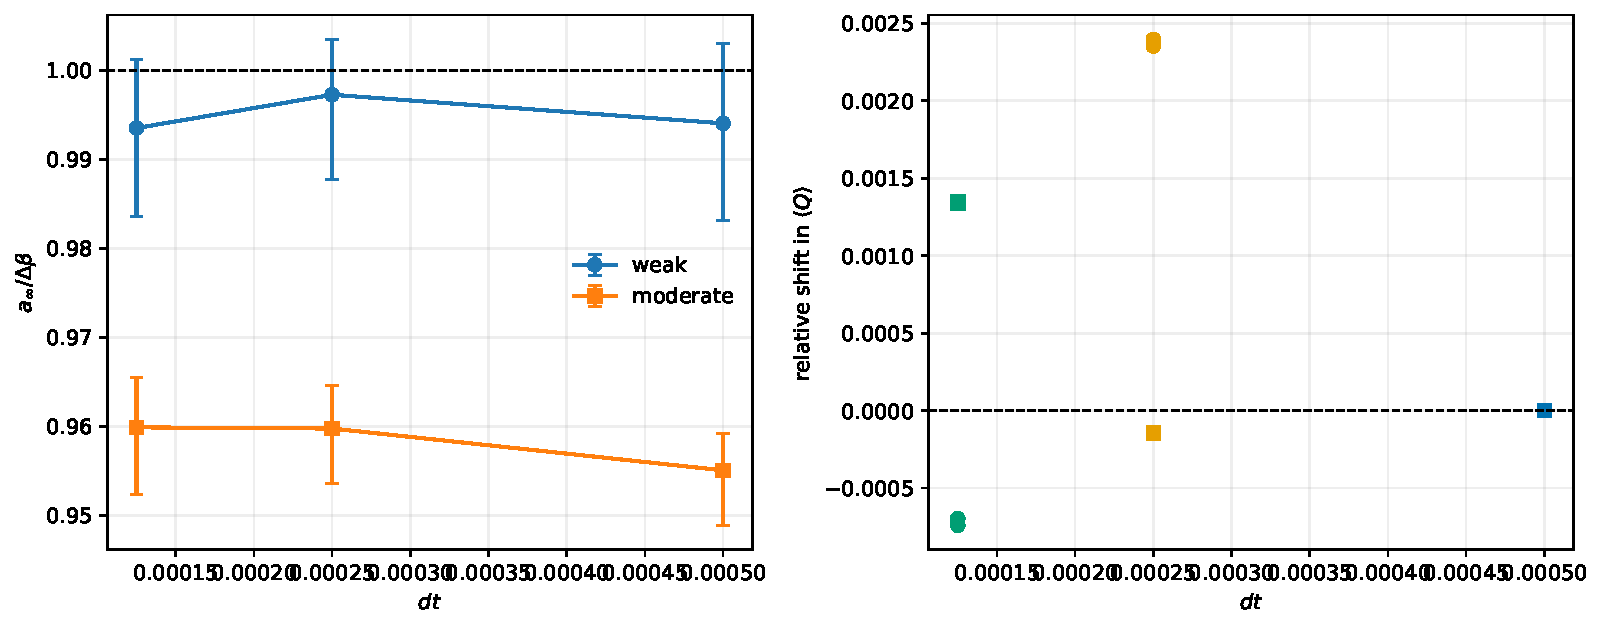
\includegraphics[width=0.98\linewidth]{../figures/timestep_summary.pdf}
\caption{Left: finite-time intercept ratios at three timesteps. Right:
relative mean-heat shifts at $\tau=5$ and 25; colours encode timestep.}
\end{figure}

\section{Finest-step three-affinity summary}
\scriptsize
\begin{longtable}{l l r r l r r c c c}
\toprule
affinity & selection & $dt$ & $a_\infty/\Db$ & 95\% CI & $\chi^2_\nu$ & max $|r|$ & adequate & CI has 1 & pass\\
\midrule
\endfirsthead
$(7,5)$ & all\_admissible & 1.250e-04 & 0.995730 & [0.988535, 1.000882] & 0.645 & 1.461 & yes & yes & yes \\
$(8,4)$ & all\_admissible & 1.250e-04 & 0.959884 & [0.952289, 0.965475] & 5.103 & 3.250 & no & no & no \\
$(6.5,5.5)$ & all\_admissible & 1.250e-04 & 0.993519 & [0.983582, 1.001209] & 0.753 & 1.703 & yes & yes & yes \\
$(7,5)$ & tau\_ge\_10 & 1.250e-04 & 1.000023 & [0.990402, 1.006965] & 0.109 & 0.528 & yes & yes & yes \\
$(8,4)$ & tau\_ge\_10 & 1.250e-04 & 0.978279 & [0.966215, 0.987892] & 0.287 & 0.884 & yes & no & no \\
$(6.5,5.5)$ & tau\_ge\_10 & 1.250e-04 & 0.994366 & [0.982963, 1.003116] & 0.863 & 1.718 & yes & yes & yes \\
\bottomrule
\end{longtable}
\normalsize

The direct finest-step criterion requires both an adequate $1/\tau$ model and
a ratio CI containing one.  An inadequate $(8,4)$ fit is reported as
unresolved rather than converted into evidence against the fluctuation
relation.

\section{Per-window results at $(6.5,5.5)$}
\begin{figure}[ht]
\centering
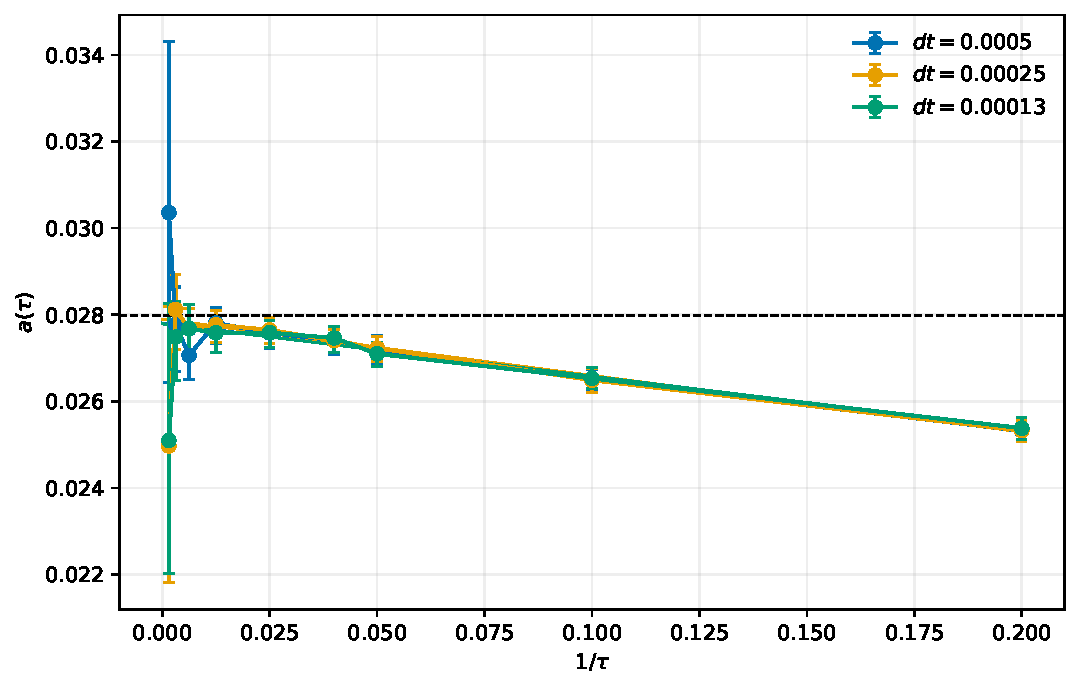
\includegraphics[width=0.72\linewidth]{../figures/finite_time_weak.pdf}
\caption{Weak-affinity finite-time slopes and frozen $1/\tau$ fits.}
\end{figure}
\scriptsize
\begin{longtable}{r r r r r r l r c}
\toprule
$dt$ & $\tau$ & $N$ & $n_-$ & pairs & $a(\tau)$ & bootstrap 95\% CI & $R^2$ & adm.\\
\midrule
\endfirsthead
5.000e-04 & 5 & 4000256 & 1747665 & 99 & 0.025317 & [0.025062, 0.025559] & 0.9979 & yes \\
5.000e-04 & 10 & 2000128 & 814568 & 84 & 0.026491 & [0.026237, 0.026743] & 0.9976 & yes \\
5.000e-04 & 20 & 1000064 & 366513 & 74 & 0.027205 & [0.026883, 0.027510] & 0.9978 & yes \\
5.000e-04 & 25 & 800000 & 280562 & 69 & 0.027407 & [0.027081, 0.027712] & 0.9976 & yes \\
5.000e-04 & 40 & 499968 & 155995 & 65 & 0.027580 & [0.027215, 0.027891] & 0.9979 & yes \\
5.000e-04 & 80 & 249984 & 60756 & 53 & 0.027806 & [0.027341, 0.028155] & 0.9979 & yes \\
5.000e-04 & 160 & 124928 & 20136 & 43 & 0.027062 & [0.026502, 0.027563] & 0.9951 & yes \\
5.000e-04 & 320 & 62464 & 5109 & 34 & 0.027776 & [0.026694, 0.028640] & 0.9944 & yes \\
5.000e-04 & 640 & 31232 & 764 & 17 & 0.030356 & [0.026423, 0.034302] & 0.9704 & yes \\
2.500e-04 & 5 & 4000256 & 1745814 & 99 & 0.025322 & [0.025081, 0.025558] & 0.9977 & yes \\
2.500e-04 & 10 & 2000128 & 813275 & 86 & 0.026487 & [0.026200, 0.026759] & 0.9978 & yes \\
2.500e-04 & 20 & 1000064 & 365872 & 74 & 0.027228 & [0.026920, 0.027503] & 0.9988 & yes \\
2.500e-04 & 25 & 800000 & 279855 & 72 & 0.027400 & [0.027117, 0.027655] & 0.9977 & yes \\
2.500e-04 & 40 & 499968 & 155701 & 65 & 0.027647 & [0.027329, 0.027934] & 0.9979 & yes \\
2.500e-04 & 80 & 249984 & 60447 & 55 & 0.027766 & [0.027365, 0.028100] & 0.9980 & yes \\
2.500e-04 & 160 & 124928 & 20012 & 44 & 0.027681 & [0.027145, 0.028150] & 0.9958 & yes \\
2.500e-04 & 320 & 62464 & 5016 & 32 & 0.028116 & [0.027188, 0.028932] & 0.9940 & yes \\
2.500e-04 & 640 & 31232 & 719 & 14 & 0.024966 & [0.021812, 0.028197] & 0.9510 & yes \\
1.250e-04 & 5 & 4000256 & 1747636 & 98 & 0.025379 & [0.025122, 0.025618] & 0.9971 & yes \\
1.250e-04 & 10 & 2000128 & 814370 & 85 & 0.026529 & [0.026294, 0.026770] & 0.9977 & yes \\
1.250e-04 & 20 & 1000064 & 366079 & 76 & 0.027095 & [0.026796, 0.027363] & 0.9982 & yes \\
1.250e-04 & 25 & 800000 & 280548 & 72 & 0.027461 & [0.027135, 0.027732] & 0.9985 & yes \\
1.250e-04 & 40 & 499968 & 156076 & 63 & 0.027584 & [0.027241, 0.027864] & 0.9978 & yes \\
1.250e-04 & 80 & 249984 & 60627 & 56 & 0.027579 & [0.027136, 0.027943] & 0.9974 & yes \\
1.250e-04 & 160 & 124928 & 20138 & 44 & 0.027680 & [0.027004, 0.028229] & 0.9967 & yes \\
1.250e-04 & 320 & 62464 & 5053 & 32 & 0.027482 & [0.026482, 0.028315] & 0.9926 & yes \\
1.250e-04 & 640 & 31232 & 781 & 15 & 0.025095 & [0.022027, 0.028266] & 0.9640 & yes \\
\bottomrule
\end{longtable}
\normalsize

\section{Per-window results at $(8,4)$}
\begin{figure}[ht]
\centering
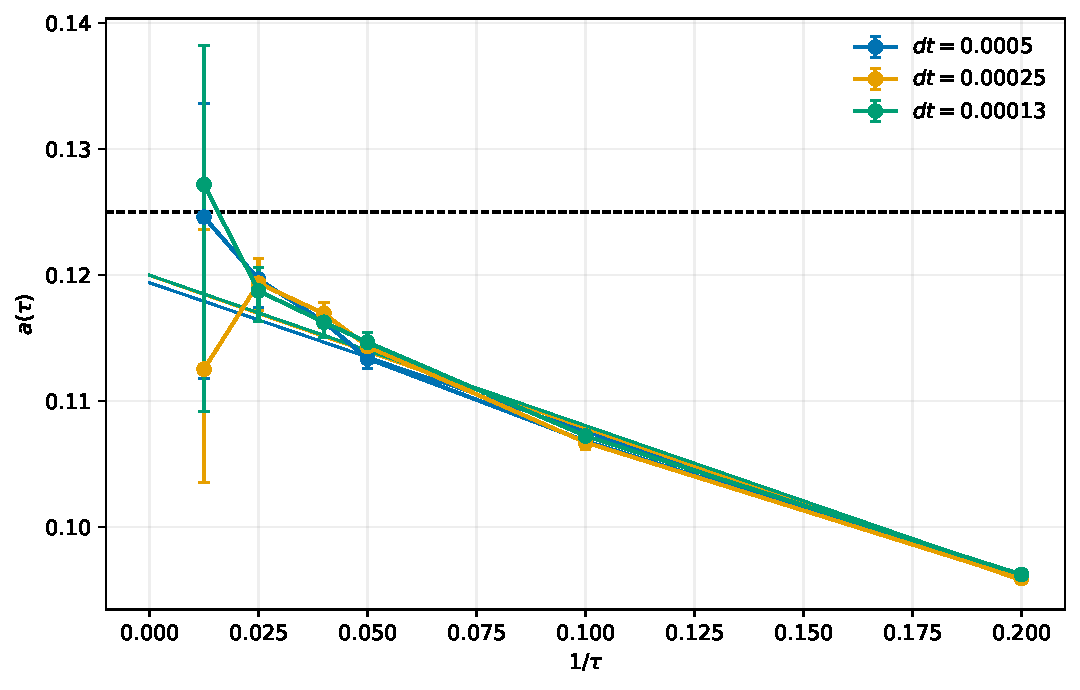
\includegraphics[width=0.72\linewidth]{../figures/finite_time_moderate.pdf}
\caption{Moderate-affinity finite-time slopes and frozen $1/\tau$ fits.}
\end{figure}
\scriptsize
\begin{longtable}{r r r r r r l r c}
\toprule
$dt$ & $\tau$ & $N$ & $n_-$ & pairs & $a(\tau)$ & bootstrap 95\% CI & $R^2$ & adm.\\
\midrule
\endfirsthead
5.000e-04 & 5 & 4000256 & 1078232 & 75 & 0.095942 & [0.095619, 0.096242] & 0.9997 & yes \\
5.000e-04 & 10 & 2000128 & 359864 & 58 & 0.106818 & [0.106332, 0.107204] & 0.9997 & yes \\
5.000e-04 & 20 & 1000064 & 88761 & 45 & 0.113369 & [0.112612, 0.114019] & 0.9995 & yes \\
5.000e-04 & 25 & 800000 & 51218 & 37 & 0.116279 & [0.115150, 0.117171] & 0.9992 & yes \\
5.000e-04 & 40 & 499968 & 12744 & 30 & 0.119661 & [0.117436, 0.121338] & 0.9975 & yes \\
5.000e-04 & 80 & 249984 & 661 & 13 & 0.124603 & [0.111797, 0.133624] & 0.9866 & yes \\
5.000e-04 & 160 & 124928 & 2 & 0 & -- & [--, --] & -- & no \\
5.000e-04 & 320 & 62464 & 0 & 0 & -- & [--, --] & -- & no \\
5.000e-04 & 640 & 31232 & 0 & 0 & -- & [--, --] & -- & no \\
2.500e-04 & 5 & 4000256 & 1078192 & 75 & 0.095897 & [0.095567, 0.096200] & 0.9998 & yes \\
2.500e-04 & 10 & 2000128 & 359207 & 58 & 0.106711 & [0.106182, 0.107191] & 0.9996 & yes \\
2.500e-04 & 20 & 1000064 & 88994 & 44 & 0.114332 & [0.113507, 0.115016] & 0.9993 & yes \\
2.500e-04 & 25 & 800000 & 51334 & 36 & 0.116946 & [0.115858, 0.117787] & 0.9993 & yes \\
2.500e-04 & 40 & 499968 & 12748 & 31 & 0.119346 & [0.117217, 0.121293] & 0.9982 & yes \\
2.500e-04 & 80 & 249984 & 646 & 14 & 0.112527 & [0.103502, 0.123602] & 0.9880 & yes \\
2.500e-04 & 160 & 124928 & 2 & 0 & -- & [--, --] & -- & no \\
2.500e-04 & 320 & 62464 & 0 & 0 & -- & [--, --] & -- & no \\
2.500e-04 & 640 & 31232 & 0 & 0 & -- & [--, --] & -- & no \\
1.250e-04 & 5 & 4000256 & 1077219 & 76 & 0.096213 & [0.095882, 0.096497] & 0.9997 & yes \\
1.250e-04 & 10 & 2000128 & 359375 & 58 & 0.107221 & [0.106663, 0.107665] & 0.9996 & yes \\
1.250e-04 & 20 & 1000064 & 88581 & 41 & 0.114660 & [0.113662, 0.115405] & 0.9995 & yes \\
1.250e-04 & 25 & 800000 & 51323 & 38 & 0.116248 & [0.115031, 0.117227] & 0.9993 & yes \\
1.250e-04 & 40 & 499968 & 12720 & 29 & 0.118734 & [0.116338, 0.120576] & 0.9986 & yes \\
1.250e-04 & 80 & 249984 & 620 & 11 & 0.127176 & [0.109144, 0.138208] & 0.9862 & yes \\
1.250e-04 & 160 & 124928 & 1 & 0 & -- & [--, --] & -- & no \\
1.250e-04 & 320 & 62464 & 0 & 0 & -- & [--, --] & -- & no \\
1.250e-04 & 640 & 31232 & 0 & 0 & -- & [--, --] & -- & no \\
\bottomrule
\end{longtable}
\normalsize

\section{Finite-time extrapolations}
\begin{landscape}
\scriptsize
\subsection*{$(6.5,5.5)$}
\begin{longtable}{r l l r l r l r r c}
\toprule
$dt$ & selection & $\tau$ used & $a_\infty$ & 95\% CI & ratio & ratio CI & $\chi^2_\nu$ & max $|r|$ & adequate\\
\midrule
\endfirsthead
5.000e-04 & all\_admissible & 5;10;20;25;40;80;160;320;640 & 0.027806 & [0.027502, 0.028057] & 0.994051 & [0.983179, 1.003040] & 1.265 & 2.380 & yes \\
5.000e-04 & tau\_ge\_10 & 10;20;25;40;80;160;320;640 & 0.027824 & [0.027482, 0.028126] & 0.994718 & [0.982477, 1.005491] & 1.466 & 2.437 & yes \\
2.500e-04 & all\_admissible & 5;10;20;25;40;80;160;320;640 & 0.027895 & [0.027630, 0.028069] & 0.997263 & [0.987776, 1.003479] & 0.700 & 1.833 & yes \\
2.500e-04 & tau\_ge\_10 & 10;20;25;40;80;160;320;640 & 0.027949 & [0.027639, 0.028172] & 0.999161 & [0.988089, 1.007162] & 0.732 & 1.865 & yes \\
1.250e-04 & all\_admissible & 5;10;20;25;40;80;160;320;640 & 0.027791 & [0.027513, 0.028006] & 0.993519 & [0.983582, 1.001209] & 0.753 & 1.703 & yes \\
1.250e-04 & tau\_ge\_10 & 10;20;25;40;80;160;320;640 & 0.027814 & [0.027495, 0.028059] & 0.994366 & [0.982963, 1.003116] & 0.863 & 1.718 & yes \\
\bottomrule
\end{longtable}
\subsection*{$(8,4)$}
\begin{longtable}{r l l r l r l r r c}
\toprule
$dt$ & selection & $\tau$ used & $a_\infty$ & 95\% CI & ratio & ratio CI & $\chi^2_\nu$ & max $|r|$ & adequate\\
\midrule
\endfirsthead
5.000e-04 & all\_admissible & 5;10;20;25;40;80 & 0.119381 & [0.118610, 0.119897] & 0.955051 & [0.948878, 0.959180] & 8.692 & 3.388 & no \\
5.000e-04 & tau\_ge\_10 & 10;20;25;40;80 & 0.121591 & [0.120402, 0.122522] & 0.972728 & [0.963220, 0.980177] & 3.466 & 2.175 & no \\
2.500e-04 & all\_admissible & 5;10;20;25;40;80 & 0.119969 & [0.119193, 0.120572] & 0.959750 & [0.953546, 0.964579] & 10.641 & 4.588 & no \\
2.500e-04 & tau\_ge\_10 & 10;20;25;40;80 & 0.122838 & [0.121468, 0.123886] & 0.982708 & [0.971741, 0.991087] & 1.776 & 1.622 & yes \\
1.250e-04 & all\_admissible & 5;10;20;25;40;80 & 0.119986 & [0.119036, 0.120684] & 0.959884 & [0.952289, 0.965475] & 5.103 & 3.250 & no \\
1.250e-04 & tau\_ge\_10 & 10;20;25;40;80 & 0.122285 & [0.120777, 0.123487] & 0.978279 & [0.966215, 0.987892] & 0.287 & 0.884 & yes \\
\bottomrule
\end{longtable}

\subsection*{$dt\to0$ diagnostics}
\begin{longtable}{l l r l r l r c c c}
\toprule
affinity & selection & $r_0$ & 95\% CI & slope & slope CI & $\chi^2_\nu$ & $O(dt)$ & all adequate & same $\tau$\\
\midrule
\endfirsthead
weak & all\_admissible & 0.995263 & [0.983447, 1.004505] & -0.280 & [-33.610, 33.700] & 0.445 & yes & yes & yes \\
weak & tau\_ge\_10 & 0.996783 & [0.982340, 1.007930] & -1.480 & [-40.151, 42.524] & 0.558 & yes & yes & yes \\
moderate & all\_admissible & 0.962499 & [0.953486, 0.969253] & -14.426 & [-35.303, 6.386] & 0.151 & yes & no & yes \\
moderate & tau\_ge\_10 & 0.983983 & [0.970072, 0.994762] & -20.410 & [-55.558, 13.708] & 1.032 & yes & no & yes \\
\bottomrule
\end{longtable}
\normalsize
\end{landscape}

The three-point $dt\to0$ lines are diagnostics.  The direct finest-step CI
and the frozen adequacy gate take priority.

\section{Mean-heat and slope shifts from $dt=5\times10^{-4}$}
\scriptsize
\subsection*{$(6.5,5.5)$}
\begin{longtable}{r r r l c r}
\toprule
finer $dt$ & $\tau$ & $\Delta a$ & bootstrap 95\% CI & contains 0 & relative $\Delta\langle Q\rangle$\\
\midrule
\endfirsthead
2.500e-04 & 5 & 4.783825e-06 & [-3.606310e-04, 3.613549e-04] & yes & 0.002396 \\
2.500e-04 & 10 & -3.485360e-06 & [-3.787527e-04, 3.709913e-04] & yes & 0.002396 \\
2.500e-04 & 20 & 2.310966e-05 & [-4.257795e-04, 4.677769e-04] & yes & 0.002396 \\
2.500e-04 & 25 & -6.918930e-06 & [-4.401585e-04, 4.225633e-04] & yes & 0.002353 \\
2.500e-04 & 40 & 6.743198e-05 & [-3.897303e-04, 5.325325e-04] & yes & 0.002339 \\
2.500e-04 & 80 & -3.945674e-05 & [-6.062809e-04, 4.959351e-04] & yes & 0.002339 \\
2.500e-04 & 160 & 6.196482e-04 & [-1.653264e-04, 0.001346] & yes & 0.002329 \\
2.500e-04 & 320 & 3.400612e-04 & [-8.427722e-04, 0.001691] & yes & 0.002329 \\
2.500e-04 & 640 & -0.005390 & [-0.010549, -6.804849e-04] & no & 0.002329 \\
1.250e-04 & 5 & 6.179599e-05 & [-2.942140e-04, 3.876489e-04] & yes & -6.966350e-04 \\
1.250e-04 & 10 & 3.821577e-05 & [-3.265993e-04, 3.627173e-04] & yes & -6.966350e-04 \\
1.250e-04 & 20 & -1.098043e-04 & [-5.341226e-04, 3.025802e-04] & yes & -6.966350e-04 \\
1.250e-04 & 25 & 5.387659e-05 & [-4.164643e-04, 4.956783e-04] & yes & -7.395775e-04 \\
1.250e-04 & 40 & 4.455938e-06 & [-4.909261e-04, 4.539484e-04] & yes & -7.381693e-04 \\
1.250e-04 & 80 & -2.263072e-04 & [-7.885918e-04, 3.928592e-04] & yes & -7.381693e-04 \\
1.250e-04 & 160 & 6.186915e-04 & [-2.568840e-04, 0.001388] & yes & -7.289794e-04 \\
1.250e-04 & 320 & -2.942128e-04 & [-0.001559, 0.001047] & yes & -7.289794e-04 \\
1.250e-04 & 640 & -0.005261 & [-0.010148, -2.100427e-04] & no & -7.289794e-04 \\
\bottomrule
\end{longtable}
\subsection*{$(8,4)$}
\begin{longtable}{r r r l c r}
\toprule
finer $dt$ & $\tau$ & $\Delta a$ & bootstrap 95\% CI & contains 0 & relative $\Delta\langle Q\rangle$\\
\midrule
\endfirsthead
2.500e-04 & 5 & -4.540900e-05 & [-4.935718e-04, 3.693904e-04] & yes & -1.406187e-04 \\
2.500e-04 & 10 & -1.070960e-04 & [-7.246587e-04, 5.377824e-04] & yes & -1.406187e-04 \\
2.500e-04 & 20 & 9.630242e-04 & [-9.530583e-05, 0.002074] & yes & -1.406187e-04 \\
2.500e-04 & 25 & 6.664523e-04 & [-7.351201e-04, 0.001974] & yes & -1.438952e-04 \\
2.500e-04 & 40 & -3.150634e-04 & [-0.003101, 0.002796] & yes & -1.384996e-04 \\
2.500e-04 & 80 & -0.012076 & [-0.025152, 0.005149] & yes & -1.384996e-04 \\
2.500e-04 & 160 & -- & [--, --] & no & -1.076552e-04 \\
2.500e-04 & 320 & -- & [--, --] & no & -1.076552e-04 \\
2.500e-04 & 640 & -- & [--, --] & no & -1.076552e-04 \\
1.250e-04 & 5 & 2.711069e-04 & [-1.756673e-04, 7.119394e-04] & yes & 0.001340 \\
1.250e-04 & 10 & 4.033429e-04 & [-2.107823e-04, 0.001042] & yes & 0.001340 \\
1.250e-04 & 20 & 0.001291 & [1.124512e-04, 0.002344] & no & 0.001340 \\
1.250e-04 & 25 & -3.138312e-05 & [-0.001474, 0.001347] & yes & 0.001346 \\
1.250e-04 & 40 & -9.271038e-04 & [-0.003782, 0.002201] & yes & 0.001347 \\
1.250e-04 & 80 & 0.002573 & [-0.016899, 0.018839] & yes & 0.001347 \\
1.250e-04 & 160 & -- & [--, --] & no & 0.001344 \\
1.250e-04 & 320 & -- & [--, --] & no & 0.001344 \\
1.250e-04 & 640 & -- & [--, --] & no & 0.001344 \\
\bottomrule
\end{longtable}
\normalsize

\section{Equilibrium estimator baseline}
\begin{figure}[ht]
\centering
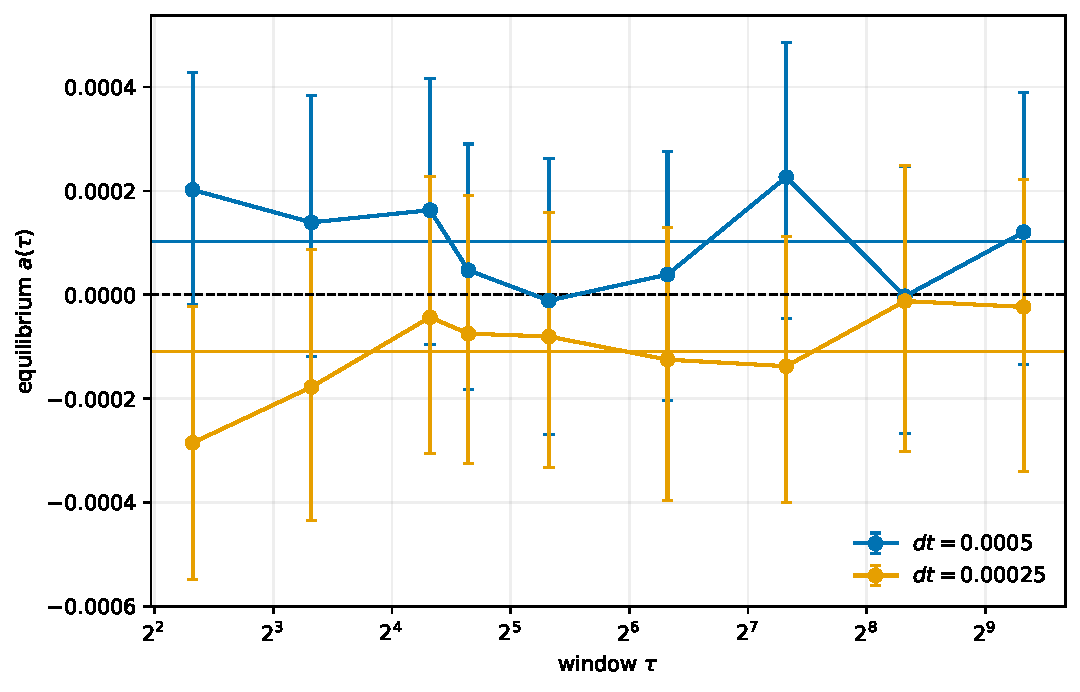
\includegraphics[width=0.72\linewidth]{../figures/equilibrium_estimator_floor.pdf}
\caption{Equilibrium per-window asymmetry slopes and their frozen weighted
means.  The exact physical reference is zero.}
\end{figure}

\scriptsize
\begin{longtable}{r r r l c r r r}
\toprule
$dt$ & $\tau$ & $a(\tau)$ & bootstrap 95\% CI & contains 0 & $n_-$ & pairs & $R^2$\\
\midrule
\endfirsthead
5.000e-04 & 5 & 2.020979e-04 & [-1.898629e-05, 4.288681e-04] & yes & 2000032 & 106 & 0.0270 \\
5.000e-04 & 10 & 1.393376e-04 & [-1.190242e-04, 3.841128e-04] & yes & 999544 & 97 & 0.0127 \\
5.000e-04 & 20 & 1.630124e-04 & [-9.526516e-05, 4.165654e-04] & yes & 499786 & 85 & 0.0214 \\
5.000e-04 & 25 & 4.721262e-05 & [-1.819332e-04, 2.903563e-04] & yes & 399455 & 81 & 0.0016 \\
5.000e-04 & 40 & -1.106779e-05 & [-2.686678e-04, 2.622487e-04] & yes & 249282 & 76 & 1.0247e-04 \\
5.000e-04 & 80 & 3.895437e-05 & [-2.037786e-04, 2.761613e-04] & yes & 124666 & 71 & 0.0010 \\
5.000e-04 & 160 & 2.266636e-04 & [-4.544486e-05, 4.860217e-04] & yes & 62425 & 66 & 0.0551 \\
5.000e-04 & 320 & -2.824073e-06 & [-2.673825e-04, 2.463902e-04] & yes & 31032 & 59 & 6.7076e-06 \\
5.000e-04 & 640 & 1.206895e-04 & [-1.337232e-04, 3.899440e-04] & yes & 15544 & 54 & 0.0124 \\
2.500e-04 & 5 & -2.850192e-04 & [-5.485820e-04, -2.332093e-05] & no & 1999557 & 107 & 0.0510 \\
2.500e-04 & 10 & -1.775594e-04 & [-4.344605e-04, 8.700647e-05] & yes & 1000353 & 94 & 0.0222 \\
2.500e-04 & 20 & -4.324976e-05 & [-3.053694e-04, 2.278426e-04] & yes & 500592 & 83 & 0.0014 \\
2.500e-04 & 25 & -7.473530e-05 & [-3.241626e-04, 1.906808e-04] & yes & 400515 & 82 & 0.0037 \\
2.500e-04 & 40 & -8.034508e-05 & [-3.324155e-04, 1.579096e-04] & yes & 250368 & 78 & 0.0052 \\
2.500e-04 & 80 & -1.248807e-04 & [-3.967967e-04, 1.291639e-04] & yes & 125167 & 70 & 0.0125 \\
2.500e-04 & 160 & -1.375052e-04 & [-3.994935e-04, 1.126236e-04] & yes & 62616 & 65 & 0.0174 \\
2.500e-04 & 320 & -1.204334e-05 & [-3.013355e-04, 2.491267e-04] & yes & 31441 & 61 & 1.8736e-04 \\
2.500e-04 & 640 & -2.336626e-05 & [-3.402746e-04, 2.227351e-04] & yes & 15729 & 56 & 6.5743e-04 \\
\bottomrule
\end{longtable}

\begin{longtable}{r r r l r l l r}
\toprule
$dt$ & weighted mean & boot. SE & 95\% CI & $z$ & $+/-/0$ & signs ($\tau$ order) & fraction of 0.057143\\
\midrule
\endfirsthead
5.000e-04 & 1.026947e-04 & 8.293064e-05 & [-5.636147e-05, 2.555512e-04] & 1.238 & 7/2/0 & +;+;+;+;-;+;+;-;+ & 0.0018 \\
2.500e-04 & -1.088285e-04 & 9.809217e-05 & [-3.069064e-04, 8.705812e-05] & -1.109 & 0/9/0 & -;-;-;-;-;-;-;-;- & -0.0019 \\
\bottomrule
\end{longtable}
\normalsize

The fine-minus-coarse equilibrium weighted baseline is
-2.115232e-04, with bootstrap SE
1.282241e-04 and 95\% CI
[-4.702495e-04, 2.809682e-05].  The two baselines
are statistically consistent under the frozen criterion.
The nominal floor is 1.088285e-04; its
ratio to the residual $(7,5)$ finest-step deficit is
0.446, which is
within
the predeclared factor-three ``same order'' range.

\section{Protocol and provenance}
The freeze/launch commit is
\path{d019ef6e3e2bd0cd149c14738ca73ee13718ffbf}.\par
The original four-case pipeline completed both $dt=2.5\times10^{-4}$ runs
but exited with status 1 after both $dt=1.25\times10^{-4}$ simulator
processes terminated before producing block CSV files.  That failure is
preserved in \texttt{pipeline.exitcode} and the
\texttt{*.initial\_failed.log} files.  The two missing fine-timestep cases
were then rerun with exactly the frozen parameters under
\texttt{RECOVERY\_AMENDMENT.md}; the recovery completed with status 0 at
\path{2026-09-13T11:56:42Z}.  The
recovery amendment was pushed as commit
\path{103cd95}.\par
Production source SHA-256:\par
\path{98e7f8f5f915c8ce02bd8aa10722025c09fd739184b981961692869c9356c0d3}.\par
Binary SHA-256:\par
\path{4c4880d721733897d200f2601690da873f5b226aaa1013df23df2351c1dfe7d1}.\par
Analysis source SHA-256:\par
\path{308d843a15fee0cce1ea589da00f3d88155d3cfb5593981d85e81d328cfa0fa7}.\par

\begin{tabular}{l l r l}
\toprule
case & kind & rows & SHA-256\\
\midrule
weak\_dt5e4 & baseline & 4000256 & \texttt{84ee7b05c008a142\ldots} \\
weak\_dt2p5e4 & new & 4000256 & \texttt{c2c81dc939a8de7f\ldots} \\
weak\_dt1p25e4 & new & 4000256 & \texttt{1b52519587878766\ldots} \\
moderate\_dt5e4 & baseline & 4000256 & \texttt{336e934df7bd8555\ldots} \\
moderate\_dt2p5e4 & new & 4000256 & \texttt{8a7df0b5ec26aba5\ldots} \\
moderate\_dt1p25e4 & new & 4000256 & \texttt{315bf4a25af37e6d\ldots} \\
equilibrium\_dt5e4 & baseline & 4000256 & \texttt{87af7c2eadcea396\ldots} \\
equilibrium\_dt2p5e4 & baseline & 4000256 & \texttt{8f5024d0d4fa0f3f\ldots} \\
\bottomrule
\end{tabular}

Exact commands and measured runtimes for the original runs are in
\texttt{COMMANDS.tsv} and \texttt{RUNTIMES.tsv}; the two recovered fine
runs are recorded separately in \texttt{RECOVERY\_COMMANDS.tsv} and
\texttt{RECOVERY\_RUNTIMES.tsv}.  The user-authorized power-policy override
is documented in \texttt{POWER\_POLICY\_OVERRIDE.md}: it changed only when
the already-running processes were allowed to execute, not any scientific
setting.  Complete per-window moments, raw symmetric-bin counts, all bootstrap
draws, residuals, and hashes accompany this report.  No scientific parameter,
estimator rule, or acceptance gate was changed after production began.

\end{document}
